\documentclass{article}
\usepackage[utf8]{inputenc}
\usepackage{amsmath}
\usepackage{algorithm}
\usepackage{enumerate}
\usepackage{algorithm}
\usepackage{algpseudocode} %[noend] %adding in no end stop the procedures ending
\usepackage{graphicx}
\usepackage{multicol} %adding tables in two columns
\usepackage{wrapfig} %adding tables in two columns
\usepackage{subfig}%adding tables in two columns
\usepackage[table,xcdraw]{xcolor}
\setkeys{Gin}{width=\textwidth}
\usepackage[mode=buildnew]{standalone}
\usepackage{placeins}
\usepackage{tikz}
\usepackage{hyperref}
\usepackage[toc,page]{appendix}
\usepackage[mode=buildnew]{standalone}

\usepackage[backend=biber, 
                url = false,
                giveninits=true]{biblatex}
%\bibliographystyle{apalike} 
\addbibresource{bibdoc.bib}

%Beyond proportional line-limits: Using physical characteristics to model line-limits in the power grid
\title{The role of proportional loading on cascading failures in the power grid}
\author{Jonathan Bourne, Elsa Arcaute, Aidan O'Sullivan}
\date{May 2018}

\begin{document}

\maketitle


\begin{abstract}
Research into cascading failures in power transmission networks requires detailed data on the capacity of individual transmission lines. However this data is often unavailable to researchers. As a result these line limits are often modelled under the assumption of being proportional to a known average load. However, there is little research into how realistic these assumptions are. In this paper, we compare the artificial line-limit method and propose an alternative model to estimate the line limit, as a linear model of length and voltage. 
We test the ability of artificial line-limits to model the true line-limits, the damage done during an attack, the order in which edges are lost and rank the relative performance of different attack strategies.
We find that the linear model is either the top performing method or close to the top in all tests. In comparison, the tolerance value that produces the best proportional loading limits changes widely depending on the test. Proportional loading was a particularly poor fit when the line tolerance was less than 2, which is the most commonly used value range in cascading failure research. The findings of this paper provide an understanding of the weaknesses of PL and provide an alternative method of line-limit modelling.
\end{abstract}


\section{Introduction}
The networked structure of power transmission grids make them susceptible to cascading failures, where the failure of a single component induces overloading and further failures throughout the network. While major blackouts are rare they affect very large numbers of people and have significant financial consequences. In 2012 a cascading failure in the power grid caused a loss of power to 600 million people \cite{Hengdao2017}. A major blackout, in the northeastern US, is estimated to have cost around USD 6 billion \cite{2014CountingUK}. These massive failures occur through cascading, and their distribution follows a power-law \cite{Dobson2004, Carreras2016, Hines2009}. A cascading failure is when a single failure or a small number of failures cause secondary failures which then spread through the system wreaking havoc. 
Given the potential magnitude of cascading failures, it is unsurprising that researchers are trying to find ways to reduce their impact and frequency. One method of understanding cascading failures is using network science. The cascading failures are stimulated using targeted attacks on network nodes or edges. There has been a lot of work in this area that focuses on developing ``vulnerability metrics" which identify the order in which nodes should be attacked to cause maximum damage to the power-grid.

When researchers first started analysing power-grids using network science the techniques applied used purely topological information about the structure of the power grid \cite{Cuadra2015}. As research developed, the electrical properties of the power-grid were incorporated creating the `Extended topology' \cite{Bompard2009}.The extended topology involves incorporating the power flowing in the network with the topological features. Electricity is transmitted through the power grid using alternating current (AC) to reduce power losses over long distances. However, as the AC power-flow equations are challenging to solve, researchers often use the Direct Current (DC) flow equations as an approximation. A recent literature review showed that 81\% of studies using power-flow use the DC approximations \cite{Cuadra2015}.
We use the DC flow calculations described by \cite{Pepyne2007} and \cite{Arianos2008}.

Many studies use synthetic networks \cite{Pepyne2007, Arianos2008, Wu2017, Hines2008} or the topological structure of a real power grid without the line-limits \cite{Yan2015, Wu2017, Buldyrev2010, Kinney2005, Schafer2018}, which are necessary in order to know of a line has tripped. Although some open data solutions are now being developed \cite{Medjroubi2017}, the lack of datasets with line-limits remains a problem.
If they are not available in the data, an estimate of the line-limits needs to be made. A common technique is to use Proportional Loading (PL). When using PL, the line-limits are set at a fixed proportion of the amount of power flowing in each line at initiation \cite{Motter, Kinney2005, Pepyne2007, Yan2015, Zhu2014, Koc2014, Ouyang2014}. Proportional Loading (PL) of networks is usually defined as $f_i^\text{max} = \alpha \left | f_{i}^c \right |$, where  $\left | f_i^c \right |$ is the absolute power-flow for line $i$ under initial conditions, $f_i^\text{max}$ is the line-limit and $\alpha$ is the tolerance factor. PL makes strong assumptions about Power-grid design for which there is no supporting evidence. There is little work using real line-limits \cite{Hines2010}, due to the, previously mentioned, difficulty of getting the datasets.

As there is no direct comparison between PL and real line-limits, it is difficult to know how accurately PL, and the simulations based on it, reflect the behaviour of the real grid, or whether a more realistic method can be created. In this paper, we address this gap. We have access to a dataset of the UK high-voltage power-grid that includes the generation and load nodes, with capacities in MW, as well as the line-limits in MW. 

We compare PL values of $\alpha$ between 1 and 50, against the real line-limits, a linear model and a topological analysis. We simulate random attacks on the power grid and analyse how well the artificial line-limits model the damage caused by the attack, and the order that edges are lost due to cascading. We also measure how well each line-limit method can rank the relative effectiveness of different grid attack strategies. The findings of this paper provide an understanding of the weaknesses of PL and provide an alternative method of line-limit modelling.

\section{Method}
The analysis was conducted in four stages. These different analyses test different aspects of how well the artificial line-limits model the real line-limits. The code used to generate the results in this paper is available on GitHub \cite{ JonathanBourne2018,JonathanBourne2018a}.

\begin{enumerate}
    \item We look at the real line-limit distribution of the network. We then compare the accuracy of PL and modelled limits against the real line-limits.

    \item We simulate random attacks on the grid, using the DC flow approximations. We attack the grid until complete collapse, repeating the process 100 times. We then compare the artificial line-limits, and real line-limits mean damage and standard deviation, at each stage of the attack.  

    \item We compare the rank order in which edges are lost due to cascades between the artificial and real line limits. we then calculate the correlation coefficient which shows us which artificial limit method most accurately represents the behaviour of grid collapse.
    
    \item To test whether the artificial line-limits can compare to vulnerability metrics, we attack the grid using five different strategies. We measure the ability of the artificial line-limits to accurately represent the true ranking of each strategy compared to the real line-limits.
\end{enumerate}

The dataset we use in this paper describes the physical and electrical structure of the UK national grid. The dataset contains 958 nodes representing substations around the UK; the nodes are connected with 1415 transmission lines which are rated 132kV, 275kV and 400kV. The network has a mean degree of 2.95 with assortivity and clustering close to zero (-0.06 and 0.03 respectively), the average unweighted nodal distance is 14.7, the mean normalised betweeness is 0.014. The dataset includes all the information required to perform the DC load flow calculations. This information includes line node connections, line reactance node load and node generation. Unusually for a power-grid dataset, it also provides line-limits making it possible to test PL. 

This paper defines the simulation parameters using 5 parameters, Physics model, Element, Attack type, Removal method and Load profile. The physics model used in this analysis is either DC flow or topological. The elements attacked are the nodes. The attack type is `fixed' meaning that the order in which the nodes will be removed is generated before the attack begins. The removal order is sequential, meaning that the node at the top of the attack order is the only node that is deliberately removed, any other nodes that are attacked that round are lost through cascading. A summary of the parameters is shown in Table \ref{tab:PEARL} The last parameter is Load profile, in this analysis we are going to use a single load profile based on the year-round base load and is provided as part of the dataset by the National Grid. These simulation parameters form the acronym PEARL, the PEARL framework is discussed in greater depth in Appendix \ref{sect:PEARL}.

    \begin{table}
\centering
\caption{PEARL settings used in this paper.}
\label{tab:PEARL}
\begin{tabular}{l|l}
Class        & Types                     \\ \hline
\textbf{P}hysics       & Cascading DC, Topological \\
\textbf{E}lement      & Node\\
\textbf{A}ttack Type  & Fixed \\
\textbf{R}emoval      & Sequential \\
\textbf{L}oad Profile & Single         
\end{tabular}
\end{table}

\subsection{Artificial line-limits and real line-limits}
To understand how artificial line-limits differ from the real line-limits we use 15 $\alpha$ values for proportional loading and also line-limits generated from a linear model. 
We use $\alpha$ values of 1.05, 1.1 1.2 1.3, 1.5, 2, 3, 5, 6, 7, 10, 15, 20, 50. The $\alpha$ values were chosen based on values used in other papers and continued until 50. The topological analysis is identical to an $\alpha$ level of infinity.

Line-limits are caused by three main factors thermal-limits in the cable, voltage drop and frequency stability. These three factors are all related to the line length and its voltage \cite{Gutman1979}. Therefore we create a linear model that uses voltage and line-length as this data is available in several open datasets  \cite{Entsoe-e, Rivera2015,OpenStreetMapcontributors2017} and the data that we have. The model has the form $y_i = \beta_0 1 + \beta_l x_{i1} + \beta_{v132} x_{iv132}+ \beta_{v275} x_{iv275}+ \beta_{v400} x_{iv400}$, where $y_i$ is the line-limit of the $i$th power-line, $x_{il}$ is the length of the $i$th power-line in Km and, $x_{iv132},\; x_{iv275}, \; x_{iv400}$ are binary vectors representing the voltage level of line $i$, the coefficients are $\beta_l, \beta_{v132}, \; \beta_{v275}, \; \beta_{v400}$ respectively, while $\beta_0$ is the model bias. 
The model is trained using ten-fold cross-validation. This model will be compared to proportional loading throughout the paper. Ideally, we would be able to use the model to predict the line-limits of a separate network. However, we only have access to the real line-limits of a single network. As this is the case, we will use the line-limits predicted in each of the folds of the validation set as the predicted line-limits for the attack simulation. The artificial line-limits are compared to the real line-limits using $R^2$, Root Mean Square Error (RMSE) and Mean Average Percent Error (MAPE). 

\subsection{Comparing Attack damage between PL and real line-limits}
We simulate the grid under attack by assigning a random node attack rank to each node in the network. We then remove the node with rank 1. As node removal can cause overloading we re-calculate the power flow and remove any lines that exceed their maximum line-limit. We then re-balance the power and load in the network. Line removal can cause the network to break into sub-components, so we remove any nodes that are in a sub-component that has no power. We then re-calculate power flow. This process c until no-further removals occur. We then find the node with the next lowest attack rank and remove it, repeating the whole process until there are no nodes left in the network. The process is described in Algorithm \ref{algo:attackthegrid} and a schematic is shown in Figure \ref{fig:AlgoSchem}.

\begin{algorithm}
\caption{Attack the grid}\label{algo:attackthegrid}
\begin{algorithmic}[1]
\Procedure {AttackTheGrid}{$G$}

\State $\mathcal{V} \leftarrow  V(G)$
\State $E \leftarrow  E(G)$

\While{$\mathcal{V} \neq \emptyset$ }
\State remove $\text{min}_i(v_i)$ 
\Comment $i$ is the order in which nodes will be attacked
\Repeat
\State calculate power flow in $G$
\For{$e \in E$}
\State  remove $e$ if $f_e > f_e^{max}$ \Comment Power flow exceeds line-limit
\EndFor
\State  re-balance generation and supply
\For{$v \in \mathcal{V}$}
\State  remove $v$ if subgraph has no power
\EndFor
\Until{ $f_e < f_e^{max}$ for all $e$}
\EndWhile
\EndProcedure
\end{algorithmic}
\end{algorithm}

\begin{figure}
    \centering
    \includestandalone[width=.8\textwidth]{CascadeSchematic}
    \caption{Schematic of the node removal process}
    \label{fig:AlgoSchem}
\end{figure}

During the attack simulation two different damage metrics will be used to analyse attack progression, these are Giant-Component size, measured as the largest connected component, and Blackout size, measured as total MW lost. They will be compared to the original state of the graph using $\Delta P_x= 1-\frac{P_1-P_x}{P_1}$, where $P_1$ is the complete graph and $P_x$ is the graph after attack $x$. This way of measuring damage returns a percentage between 0 (no damage) and 100\% (complete grid collapse).

Using the largest connected component as a measure might not be representative of the physical processes that occur on the power grid. For example, a network that has 100 nodes but only 2 generators, where the first generator produces 99\% of the electricity and the other generates the remaining 1\%. If the big generator fails, the giant-component size is still 99\% indicating that the network is almost unaffected, even though there only is 1\% of the necessary power. Despite this drawback, the simplicity of the metric has made it a popular choice \cite{AndreaPagani2014, Motter, Rosas-Casals2007,Pagani2011} and so will be included here.
Blackout size is a metric from the extended topology. It measures the amount the loss of system power in MW. This metric is popular and has several different names with slightly different implementations but which produce a similar result. It has been called Loss of Load \cite{Wang2011}, Blackout size \cite{Hines2010}, Load shed \cite{Carreras2016}, Power Supply \cite{Ouyang2014}, Total Loss of Power \cite{BrancucciMartinez-Anido2012} among others. This metric does not suffer the same problem described for the size of giant component.

\subsection{Comparing the order in which edges are lost due to cascade}
Although accurately modelling the damage done in an attack provides much insight into the vulnerability of a grid, sometimes it is useful to know the order in which nodes or edges were lost for the purposes of either network or node vulnerability metrics \cite{Yang, Hines2017, Zhu2014}. However, if the order of the nodes being lost differs depending on the line-limits then the results of such analyses will not be reliable. To explore the robustness of loss order in relation to line-limits we correlate the order in which nodes are lost during an attack for artificial line-limits with the real line-limits.

Tables \ref{table:SimAttackOrder} and \ref{table:NodeLossOrder} give a toy example of how we compare node loss order. First n node removal orders are generated. Then all n simulations are run using each line limit type. Table \ref{table:NodeLossOrder} shows simulation 1 for the Real line-limits and a line-limit of $\alpha = 3$. In the table yellow cells indicate that a node was targeted for removal, whilst the other nodes were lost due to the cascade. We find the similarity of network collapse by correlating the round lost to cascade of the nodes, this means we exclude nodes that were targeted for removal. In the example that means that only nodes F, G and H can be compared.

We use the Spearman's correlation $\rho_n = \frac{\text{cov}(\text{rg}_{x,n},\text{rg}_{y,n})}{\sigma_{\text{rg}_{x,n}}\sigma_{\text{rg}_{y,n}}}$, where $\text{rg}_{x,n}$ and $\text{rg}_{y,n}$ are the rank of $x_n$ and $y_n$ respectively. In this case, $x_n$ is the vector of node removal rounds of the artificial line-limit for simulation $n$ and $y_n$ is the vector of node removal round for the real line-limits for simulation $n$. In the example this means $x_n = {2,4,4}$ and $y_n = {1,3,2}$ giving a correlation of 0.866. 

In this experiment we generate 100 attack orders for the 958 nodes producing 100 correlation scores per line-limit method. We can then see how similar the collapse order of the artificial line-limits are to the real line-limits.

\iffalse
The attack round in which each edge was removed (either by direct attack or cascade) is recorded up until the grid has completely collapsed. We the calculate the correlation coefficient between the artifical line-limits and real line-limits. The higher the correlation, the more accurately the artificial line-limit can model the collapse behaviour of the real grid. As the data is not normally distributed, we will use the Spearman's correlation $\rho_n = \frac{\text{cov}(\text{rg}_{x,n},\text{rg}_{y,n})}{\sigma_{\text{rg}_{x,n}}\sigma_{\text{rg}_{y,n}}}$, where $\text{rg}_{x,n}$ and $\text{rg}_{y,n}$ are the rank of $x_n$ and $y_n$ respectively. In this case, $x_n$ is the vector of edge removal rounds of the artificial line-limit for simulation $n$ and $y_n$ is the vector of edge removal round for the real line-limits for simulation $n$. The length of $x$ and $y$ is 1415 which is the total number of edges.

\fi

\begin{table}
\parbox{.45\linewidth}{
\centering
\label{my-label}
\begin{tabular}{l|llll}
\begin{tabular}[c]{@{}l@{}}Node\\ ID\end{tabular} & Sim 1 & Sim 2 & $\cdots$ & Sim n \\
\hline \\
A       & 1     & 4     & $\cdots$ & 3     \\
B       & 2     & 2     & $\cdots$ & 8     \\
C       & 3     & 1     & $\cdots$ & 7     \\
D       & 4     & 6     & $\cdots$ & 6     \\
E       & 5     & 5     & $\cdots$ & 1     \\
F       & 6     & 7     & $\cdots$ & 2     \\
G       & 7     & 8     & $\cdots$ & 5     \\
H       & 8     & 3     & $\cdots$ & 4    
\end{tabular}
\caption{The Node removal orders are randomly generated n times.}
\label{table:SimAttackOrder}
}
\hfill
\parbox{.45\linewidth}{
\centering

\begin{tabular}{l|lll}
\begin{tabular}[c]{@{}l@{}}Node\\ ID\end{tabular} & Sim 1& \begin{tabular}[c]{@{}l@{}}Real\\ Limits\end{tabular} & $\alpha = 3$              \\
\hline \\
A       & 1                                                      & \cellcolor[HTML]{FCFF2F}1                             & \cellcolor[HTML]{FCFF2F}1 \\
B       & 2                                                      & \cellcolor[HTML]{FCFF2F}2                             & 1 \\
C       & 3                                                      & 1                                                     & \cellcolor[HTML]{FCFF2F}2                         \\
D       & 4                                                      & \cellcolor[HTML]{FCFF2F}3                             & \cellcolor[HTML]{FCFF2F}3 \\
E       & 5                                                      & \cellcolor[HTML]{FCFF2F}4                             & 1                         \\
F       & 6                                                      & 2                                                     & 1                         \\
G       & 7                                                      & 4                                                     & 3                         \\
H       & 8                                                      & 4                                                     & 2                        
\end{tabular}
\caption{Yellow nodes were targeted for removal and so are not included when calculating removal similarity.}
\label{table:NodeLossOrder}
}
\end{table}




\subsection{Comparing vulnerability rankings accuracy}


The choice of attack strategy can have substantial impact on results, different strategies will damage the network at different rates throughout the attack. When comparing attack strategies, it may be that only the relative performance is important. In this analysis we compare the ability of different line-limit methods to accurately rank attack strategies. We compare 5 different attack strategies across 8 $\alpha$ values and the modelled limits as well as the topological limits. The $\alpha$ values used in this analysis are 1.05, 1.1,1.5, 2, 5,  10, 20, 50.

The attack strategies that we will use in this analysis are a mixture of topological methods and also extended topology. The strategies are Entropic degree \cite{Bompard2009} using line-limit, Entropic degree \cite{Bompard2009} using initial power flow, Degree, Centrality and Electrical Centrality \cite{Wang2011}.

Using each attack strategy to define the node removal order, we simulate an attack to grid collapse. After each attack round (node removed) we rank the strategies by total blackout size. This means that the strategy that has caused the most damage to the network gets rank 1 and the strategy that has caused the least damage gets rank 5. We then compare the rankings obtained by each artificial limit with the real line-limits. Using RMSE, we evaluate which line-limit method has the lowest error relative to the real line-limits.

\section{Results}
The results are split into two sections. The first section describes the results of the linear model used to generate line limits, the second section compares the performance of the different artificial line-limits to the real line-limits

\subsection{Modelling line-limits}
We first create a linear model that predicts line-limits. The variables used are Voltage and line-length in kilometers, the network is represented in Figure \ref{fig:VoltageMap} using geographical location in the UK and a graph space representation using force expansion.  As we only have a single network we use 10-fold cross-validation to train on 90\% of the data then predict using the remaining 10\%. The model coefficients are quite stable, see Table \ref{tab:ModCoeffs}. The mean intercept across the ten folds was 590MW,  the line-limit increases 1 MW per kilometre of power line. When a line is 132Kv it reduces the predicted line-limit by 440MW whilst lines of 275KV increase the line-limit by 258MW and the highest voltage 400kv lines increase the line limit by 1673MW. These findings are intuitive as longer lines and higher voltages are more likely to carry larger amounts of power.

\input{Figures/ModCoeffs.txt}

\begin{figure}
    \centering
    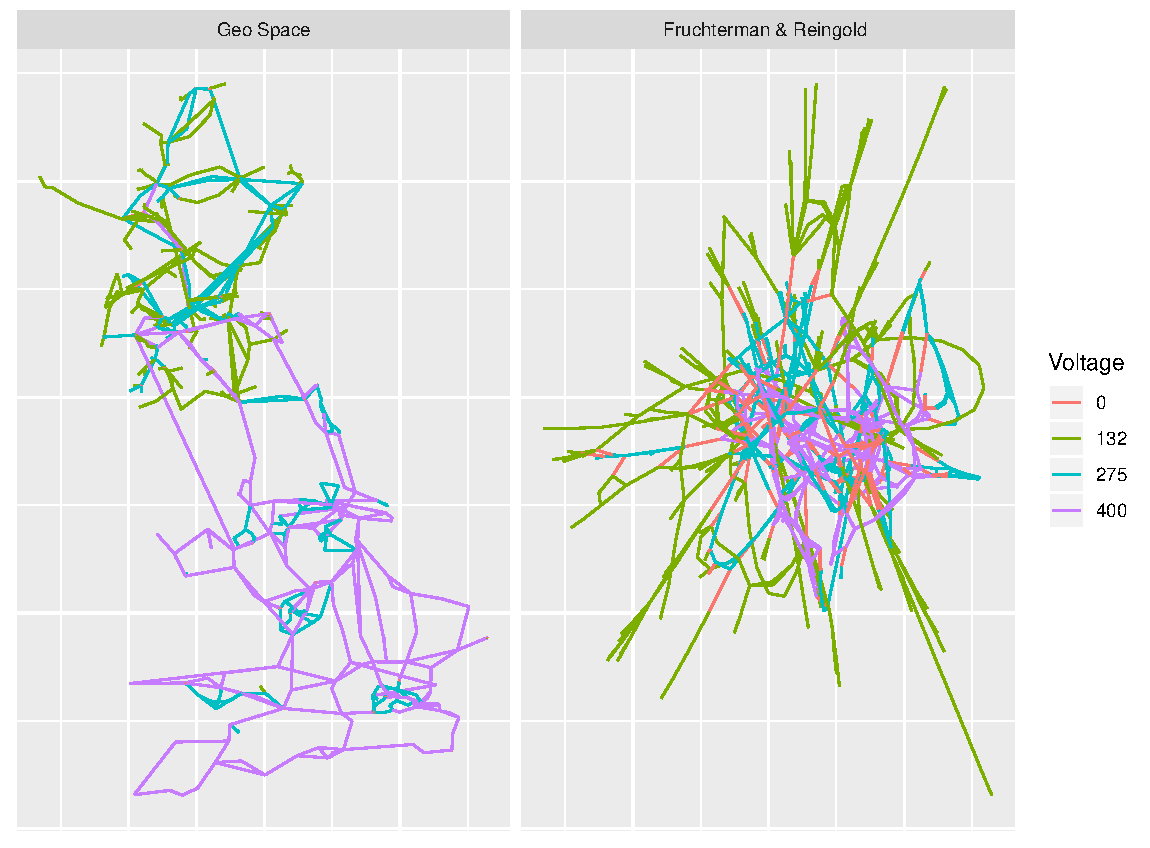
\includegraphics{Figures/ggMapColouredEdges.pdf}
    \caption{UK power-grid voltage level shown in geographical space and graph space}
    \label{fig:VoltageMap}
\end{figure}

\subsection{Comparing the performance of different line-limits}

Inspection of the distribution of the power-grid tolerance under initial conditions shows that the system is not proportionally loaded. Figure \ref{fig:LoadLevel} shows the $\alpha$ distribution  of the power grid under initial loading. The power grid has a mean $\alpha = 5.4$ and a median $\alpha = 6.13$ These tolerances are much higher than those used in the literature which are typically less than 2.

Correlating PL limits with real limits shows an  $R^2$ of 0.45. Using a range of $\alpha$ values, we find that the minimum MAPE and RMSE are 0.54 and 893 with $\alpha$ values of 3.6 and 3.3 respectively. In contrast, the linear model outperforms all $\alpha$ values having an $R^2$, MAPE and RMSE of 0.79, 0.50 and 437 respectively.

\begin{figure}
    \centering
    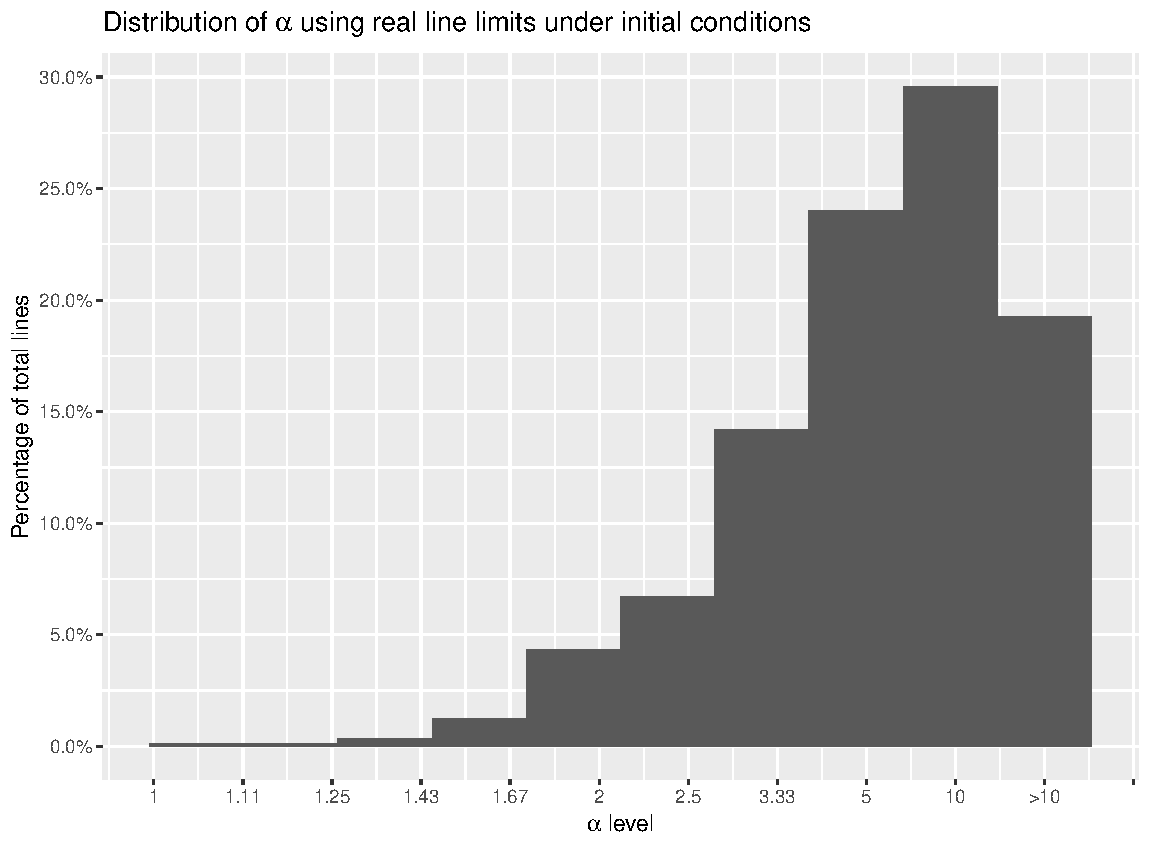
\includegraphics{Figures/LoadLevel.pdf}
    \caption{The distribution of the loading is left skewed with a mean $\alpha$ of 5.4.}
    \label{fig:LoadLevel}
\end{figure}

We explore the damage done during random attack across different values of alpha. We see that that alpha has a logarithmic relationship with the damage for a given number of attacks. Figure \ref{fig:DamageDone} shows that for both damage metrics the $\alpha$ levels only converge at grid collapse and do not cross each other before that.

We also see that only a few $\alpha$ levels are in the same region of the real line-limits. When looking at blackout size, $\alpha = 5$ minimises the RMSE between PL and the real line-limits with an RMSE of 0.042, see Figure \ref{fig:RMSEchange}. The next best fit is $\alpha = 6$ with an RMSE of 0.057 followed by the linear model with an RMSE of 0.066. 
For the giant-component, $\alpha=10$ minimises the RMSE with a value of 0.012, followed by the linear model with an RMSE of 0.042.

The error relationship between blackout size and optimum $\alpha$ is intuitive as it matches the average $\alpha$ of the real line-limits. The reason for the giant-component optimum $\alpha$ is less apparent but is probably linked to the topological structure. However, the linear model is a high performer with both damage metrics.

Next, we compare the standard deviation of damage across all 100 simulations. The linear model has the best fit for the standard deviation of the blackout size, with an RMSE of 0.023, followed by $\alpha = 3$ which has an RMSE of 0.032. The accuracy of the linear model comes from its ability to represent the hump of the real limits shown in Figure \ref{fig:SDDamage}, something that no value of $\alpha$ can replicate.

When looking at the RMSE of the standard deviation of the damage of the giant-component, we see that $\alpha = 10$ minimises the error with an RMSE of 0.011. The linear model is the second-best performer with an RMSE of 0.018. 

\begin{figure}
    \centering
    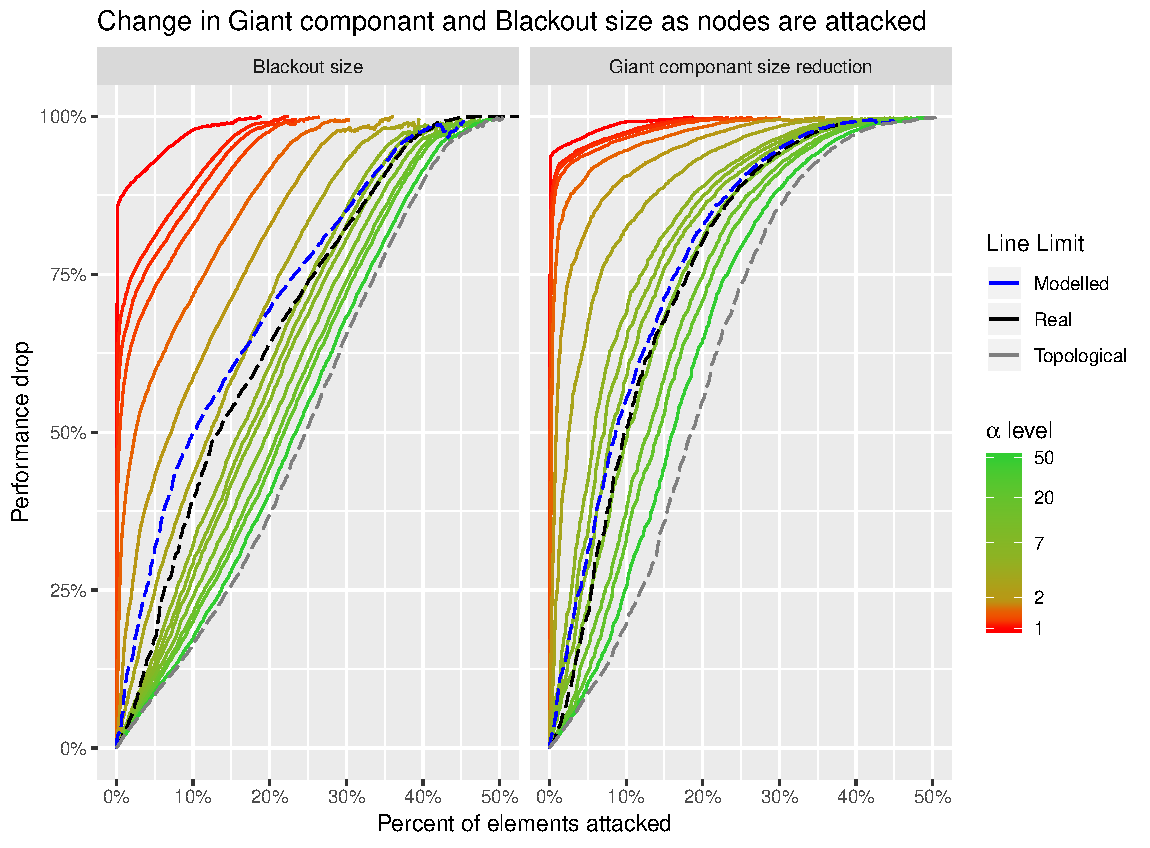
\includegraphics{Figures/GCandBlackoutChange.pdf}
    \caption{Mean damage done in terms of giant component and blackout size across 100 simulations, across all 15 $\alpha$ levels and the linear model. There is a log relationship between $\alpha$ and damage done for a given number of elements attacked.}
    \label{fig:DamageDone}
\end{figure}


\begin{figure}
    \centering
    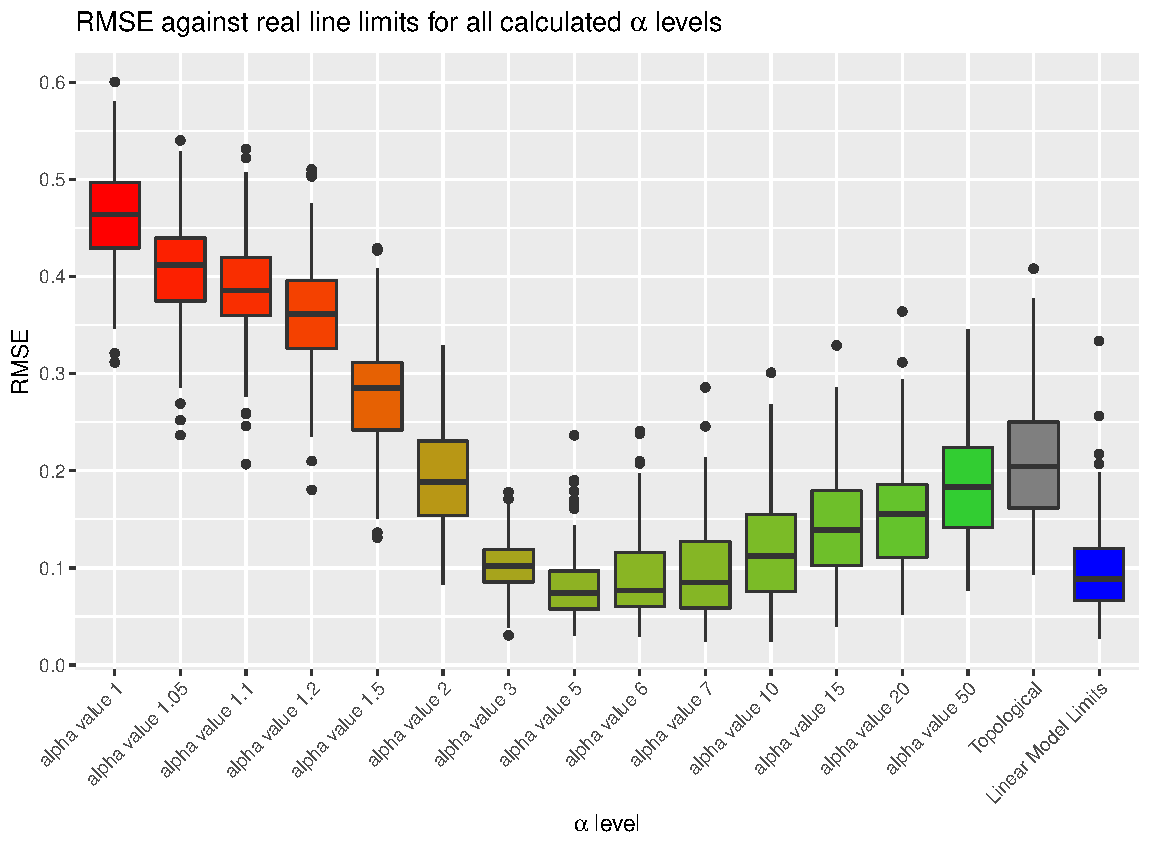
\includegraphics{Figures/RMSEChange.pdf}
    \caption{The RMSE between the real limits and PL is minimised when PL matches the average $\alpha$ of the real system. However, the RMSE of the linear model comes a close second.}
    \label{fig:RMSEchange}
\end{figure}

\begin{figure}
    \centering
    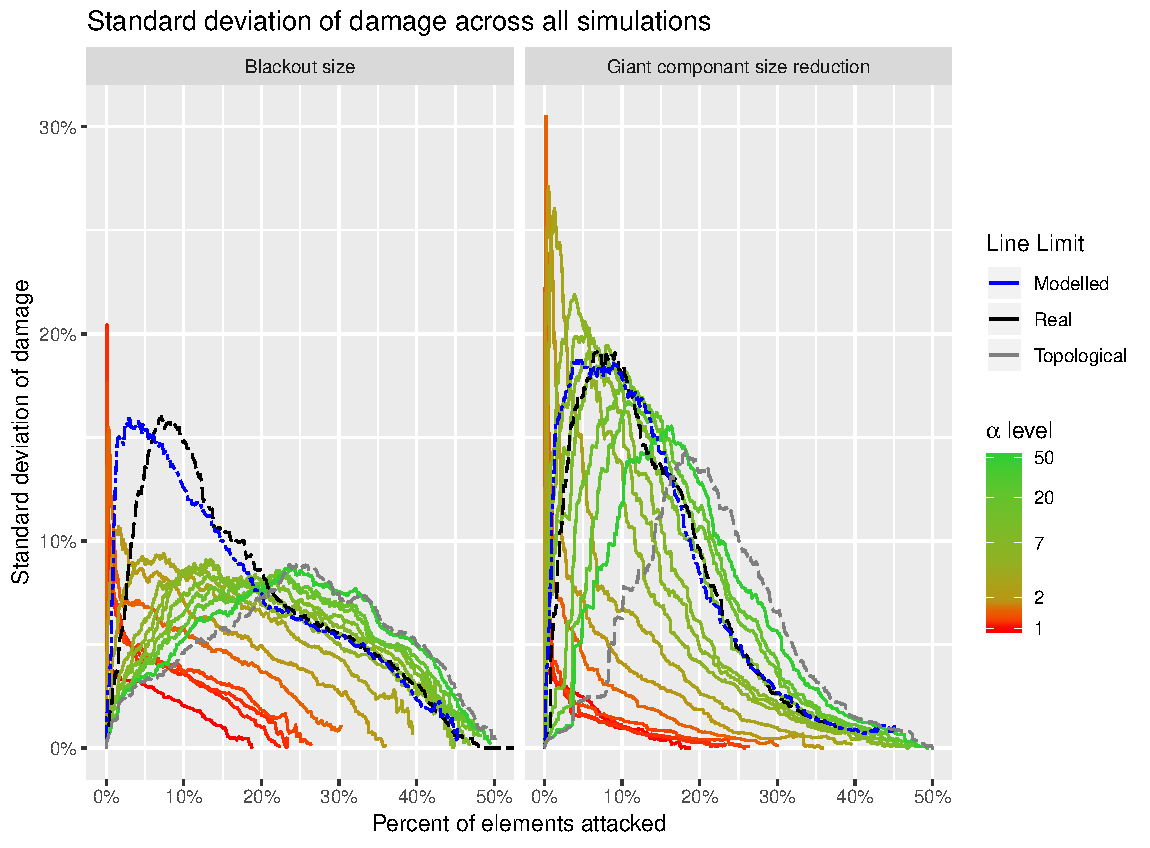
\includegraphics{Figures/SDchange.pdf}
    \caption{The standard deviation of the attack damage across the 100 simulations.}
    \label{fig:SDDamage}
\end{figure}

We compared the correlation of the order of node loss between each artificial line-limit and the real line-limits. The correlation across all 100 simulations is shown in Figure \ref{fig:DamCor}. The figure shows that as $\alpha$ increases the node loss order similarity increases following a logarithmic growth curve with a maximum at the topological analysis. The topological analysis has a mean correlation of 0.848, more than four times higher than $\alpha = 1.05$ which has a mean of 0.196. Once again the linear model beats all $\alpha$ values having a mean correlation of 0.882. Having the highest correlation value means that the linear model most accurately represents the order in which nodes are lost during an attack.

\begin{figure}
    \centering
    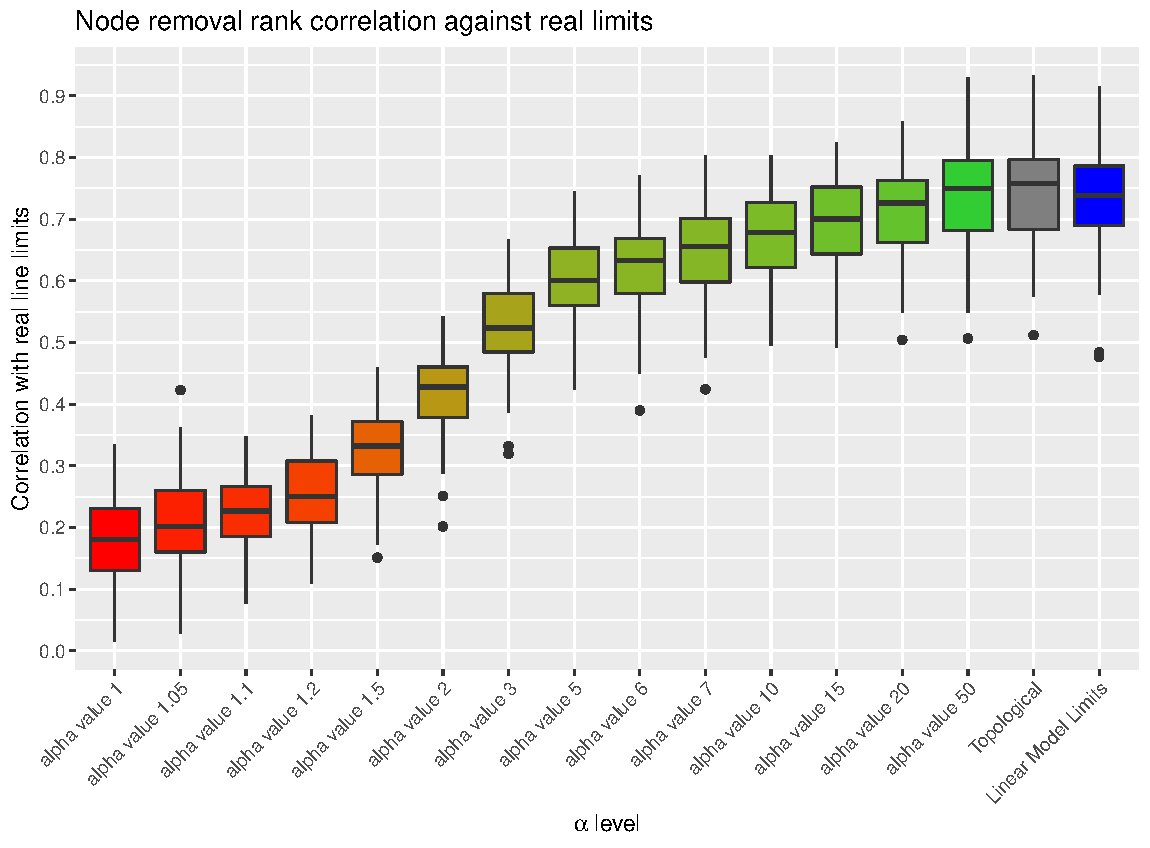
\includegraphics{Figures/CorBoxPlot.pdf}
    \caption{The linear model has the highest mean value. Correlation of edge removal increases as $\alpha$ tends to infinity which is identical to a topological analysis.}
    \label{fig:DamCor}
\end{figure}


Figure \ref{fig:AttackStratDiff}, shows plots of the damage caused by the five attack strategies in 4 of the ten different line-limit scenarios. As can be seen, the rankings of the attack strategies change as the number of nodes removed increases.
We analyse how well each line-limit method reflects the relative performance of the attack strategies. We find that the linear model is outperformed by all $\alpha$ values between 10 and 50, as well as the topological analysis, although the difference is small see Figure \ref{fig:AttackStratRankPerf}. Values of $\alpha$ that are less than or equal to 5 have a considerably greater error in ranking different attack strategies. 

That the low $\alpha$ values are much worse at ranking the performance of attack strategies is important as the majority of proportional loading papers use $\alpha$ values of less than 5. One reason for this may be that with lower $\alpha$ values the cascade size is bigger.

\begin{figure}
    \centering
    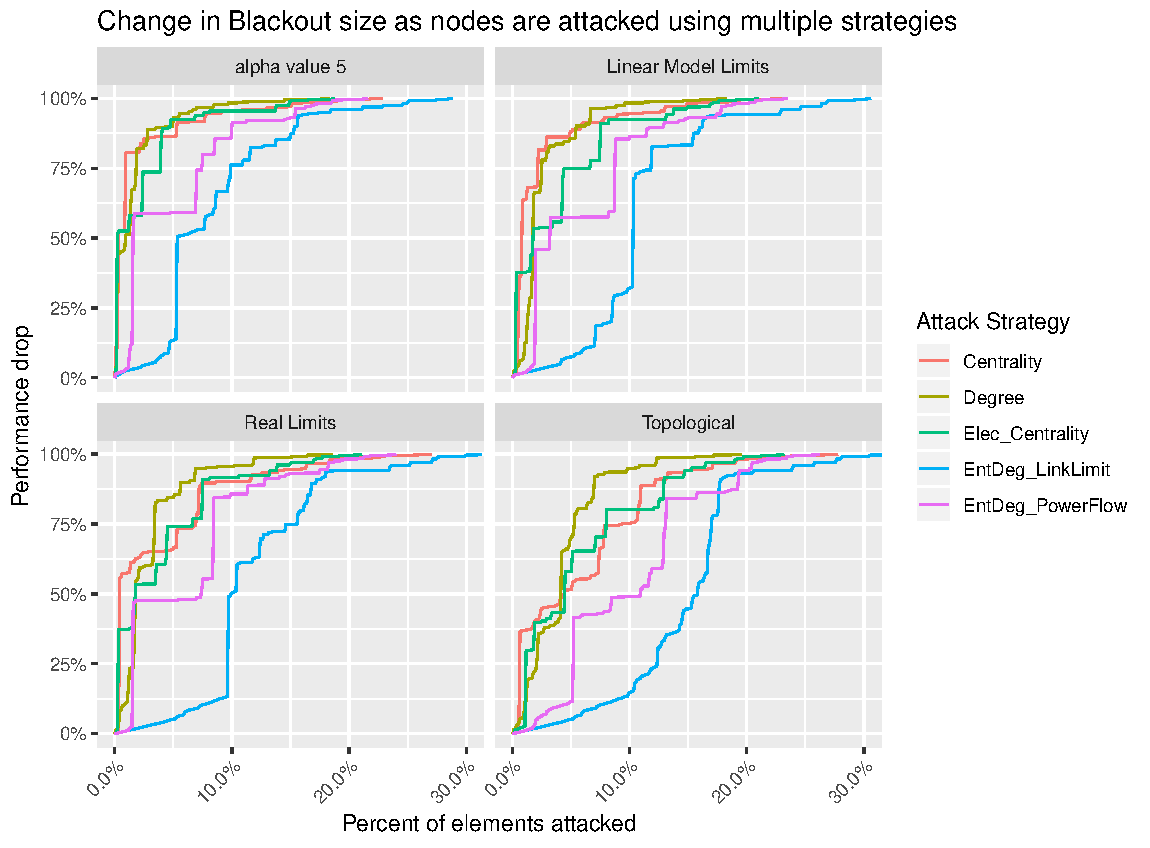
\includegraphics{Figures/AttackStratDiff.pdf}
    \caption{The figure shows the damage done to the power grid by each attack strategy by percentage of the grid attacked. As can be seen strategy rank can change as a higher percentage of nodes are removed.}
    \label{fig:AttackStratDiff}
\end{figure}


\begin{figure}
    \centering
    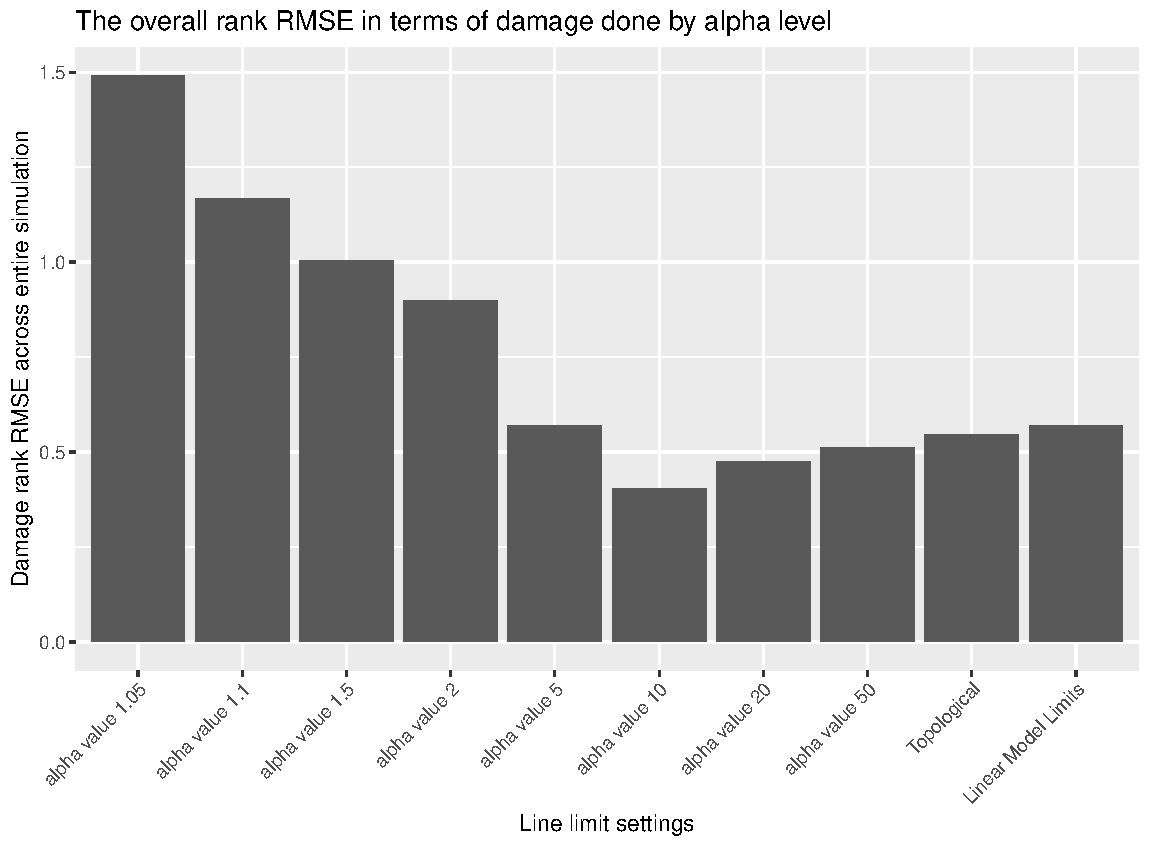
\includegraphics{Figures/AttackStratRankPerf.pdf}
    \caption{The $\alpha$ values above 5 and the linear model all have a similar performance. The $\alpha$ values below two are particularly poor at ranking attack strategies.}
    \label{fig:AttackStratRankPerf}
\end{figure}



\iffalse
The TSNE plot and random forest support the findings in Figure \ref{fig:DamCor}. The TSNE plot shows that there is considerable overlap between close $\alpha$ levels and only $\alpha$ levels which are logarithmically close to infinity, in Figure \ref{fig:DamageDone}, are close to the real line-limits. The random forest, see Table \ref{tab:ConfusionForest}, shows that there is some difficulty separating nearby $\alpha$ levels but not when the difference in $\alpha$ is large. 


\begin{figure}
    \centering
    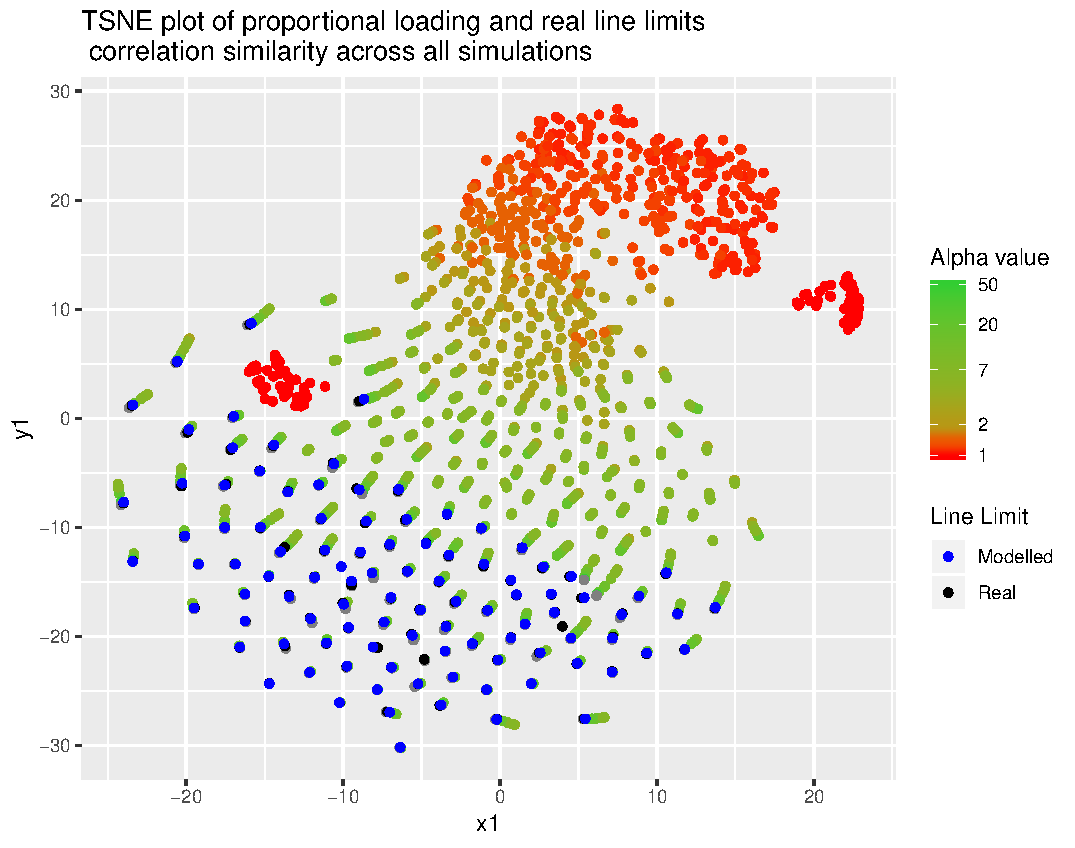
\includegraphics{Figures/TSNEcor.pdf}
    \caption{The low dimensional representation of the correlation of edge removal. The plot shows the intuitive result that $\alpha$ levels correlate most strongly with similar $\alpha$ levels}
    \label{fig:TSNE1}
\end{figure}

\input{Figures/ModelPerformance.txt}
\fi

\section{Discussion}

This paper has found that using a linear model to estimate line-limits of a power grid is a consistently high performer with one of the lowest errors across a variety of tests. The linear model produces the lowest RMSE regarding modelling the actual limits. What's more, it is in the top 3 of all results apart from the attack strategy performance ranking. However, when calculating the relative rank of attack strategies, the difference is small between all $\alpha \geq 5$ and the linear model.
We find that the optimum $\alpha$ level is not consistent and changes depending on what is being measured although the system mean $\alpha$ of 5 performed well, sometimes other values such as 3, 10, 20 or the topological analysis were the best performing method in specific analyses. 

Results based on these lower values of $\alpha$ may conclude that the risk of cascading blackouts in some networks is greater than it actually is and give a false indication of the robustness of power networks to cascading failure. 


\iffalse
Values of $\alpha$ that were less than two had particularly poor results; this is important as the majority of proportional loading research uses values in this region.

These substantial differences in $\alpha$ performance compared with the stable high performance of the linear model indicate that a replacement for proportional loading is necessary to ensure that research on cascading failures in the power grid is accurate and reliable. 
Before such a method is developed, the upmost care should be taken when selecting an $\alpha$ value so that it produces the most accurate result for the research question.
\fi


\printbibliography
\newpage
%\appendix
\begin{appendices}

\section{Defining the simulation using the PEARL framework}  
\label{sect:PEARL}
Understanding the parameters of a simulation is essential to understanding how a simulation works. A lack of data on the relative behaviour of different simulation methods makes it difficult to compare the results of different studies. To better understand simulation output , simulation parameters need to be clearly defined. Table \ref{tab:SimuParamsABS} gives a taxonomy of the simulation parameters used to define the experiments. The subsequent subsections define each of the parameters and also the options that are implemented in the R Power grid Networking package \cite{JonathanBourne2018a}. The simulation parameters proposed are not meant to be exhaustive but do describe key areas where clarity over simulation strategy helps interpret the results and replicate the experiment.  N.B the attack strategies are deployed within a simulation and are not a part of the parameters.

    
\begin{table}[ht]
\centering
\caption{Classifications}
\label{tab:SimuParamsABS}
\begin{tabular}{l|l}
Class        & Types                     \\ \hline
Attack Type  & Fixed, Flexible, Adaptive \\
Physics Model      & Cascading DC, Topological \\
Removal Regime     & Sequential, Simultaneous, hybrid  \\
Target Element      & Node, Edge, Both        \\
Repetition Method & None, Random , Timeseries sampling, Random load        
\end{tabular}
\end{table}

\subsection{Physics}

The physics model is usually the most well-defined part of the simulation as it is the rule structure under-which nodes and edges will operate. Line flow limits and balancing method are included as part of the physics model. Although there are many different physics models, in this package I consider only two.

\begin{itemize}
    \item Cascading DC: This model uses DC flow calculations to decide whether the line-limits have been exceeded. This method can lead to cascading failures as power is redistributed across the network.
    \item Topological: This is a purely topological view of the power grid in which cascades are not possible. Although there are no cascades, multiple nodes can be lost in a single attack by islanding on a component doesn't have both load and generation. A topological analysis is equivalent to proportional loading when $\alpha = \infty$
\end{itemize}

\subsection{Element}
Are Nodes, Edges, or both being targeted during this attack? Certain attack strategies, such as degree, only work one element type, while others can be applied to both, e.g. Net-ability \cite{Arianos2008}.

\begin{itemize}
    \item Nodes: Attack strategies will only consider nodes
    \item Edges: Attack strategies will only consider edges
    \item Both: Attack strategies will consider both nodes and edges. Can only be used for certain metrics
\end{itemize}


\subsection{Attack Type}
\label{sect:attacktype}
The attack type defines how an attack strategy will be executed. There are two classes of attack type, single calculation and repeated calculation. For single calculation, the attack order is calculated once before the attack begins. Repeated calculation only finds the next node to be removed and is calculated again every attack round. Below the different attack types are defined.

\begin{itemize}
    \item Fixed: This single calculation method produces a target vector of $n$ nodes for removal. If some of those nodes are lost before being targeted, then the total amount of nodes targeted for removal will be $k-f$. Where $f$ is the total number of nodes lost due to cascades or islanding
 
    \item Flexible: This single calculation method produces a target vector of $k$ nodes for removal then removes $n$. This attack type is different from the Fixed method as it will always remove $n$ nodes, as long as the graph still has nodes to remove. If $n=20$ and the 19th node is lost in a cascade, the 21st node will be added to the target list.

    \item Adaptive: This is a repeated calculation with the node order being re-calculated at every attack. This attack type allows the order of removal to change as an attack develops. In a degree based attack after a few node removal rounds some previously high degree nodes may have lost several neighbours. In contrast, other loads may not have lost any neighbours and be relatively more important.
\end{itemize}

\subsection{Removal Regime}

The removal regime describes how nodes or edges will be removed from the network. The regime has implications if the physics model allows cascades. However, removal regime has less affect on non-cascading simulations.

\begin{itemize}
    \item Sequential: The nodes on the target list are removed sequentially. The resulting cascades (if applicable) are calculated, and the grid is stabilised before the next node is removed
    \item Simultaneous: The nodes in the target list are removed at the same time. This only makes sense when $k \gg n$
    \item Hybrid: The nodes are removed in small groups, but the groups are removed sequentially. As an example 30 nodes will be removed however they be removed in 3 groups of 10
\end{itemize}

\subsubsection{Load Profile}

In many simulations, samples are taken to find a representative final result. In such cases how the samples are chosen needs to be defined.

\begin{itemize}
    \item None: The most straightforward only a single attack run is made for each strategy using a given load profile
    \item Random: Only useful for the random attack strategy. The attack is repeated multiple times, and the results averaged. In most other attack strategies the results will be identical
    \item Time series sampling: When a time series of loads are available for a network, it is randomly sampled to produce a variety of load profiles. Attacks can then be performed across the multiple time points, and the results analysed
    \item Random Load: Several papers have some variant of randomly assigning loads and generation across the network and then simulating attack. This method can only be used when line-limits are proportional to initial loading
\end{itemize}



\iffalse
\section{Computational Details}
\label{App:CompDet}
This paper uses a proprietary dataset that cannot be released into the public domain. However reproducible code and an artificial dataset are available at the link below. A link is also provided for the R package developed as part of this paper.


The code for this paper can be found here
\begin{itemize}
    \item https://github.com/JonnoB/ProportionalLoading
\end{itemize}

The code for the R package can be found here
\begin{itemize}
    \item https://github.com/JonnoB/PowerGridNetworking
\end{itemize}
\fi

\end{appendices}


\end{document}
